% \section{Error Analysis}
% \label{app:error-analysis}

% % % \begin{table*}[t]
% % \centering
% % \small
% % \setlength{\tabcolsep}{5pt}
% % \begin{tabular}{lccccc}
% % \toprule
% % \textbf{Model}
% % & \textbf{Failed runs}
% % & \textbf{No Traction}
% % & \textbf{Irrecoverable Drift}
% % & \textbf{Weak Recovery}
% % & \textbf{Interaction Breakdown} \\
% % \midrule
% % \textit{GPT-5.4} & 152 & 7.2 & 69.1 & 5.9 & 13.2 \\
% % \textit{DeepSeek-V4-Flash} & 120 & 2.5 & 21.7 & 3.3 & 71.7 \\
% % \textit{Gemini-3.5-Flash} & 153 & 13.1 & 60.1 & 3.3 & 7.8 \\
% % \textit{Llama-3.3-70B-Instruct} & 265 & 10.9 & 35.1 & 0.4 & 52.5 \\
% % \midrule
% % \textbf{All models} & 690 & 9.1 & 45.8 & 2.8 & 37.2 \\
% % \bottomrule
% % \end{tabular}
% % \caption{Default-setting trajectory failure categories (\% of failed runs). A successful call is counted as progress if it produces a new intermediate value needed by at least one valid tool-use path toward the final answer.}
% % \label{tab:mechanistic_navigation_breakdown}
% % \end{table*}

% \begin{table*}[t]
% \centering
% \small
% \setlength{\tabcolsep}{5pt}
% \resizebox{\linewidth}{!}{
% \begin{tabular}{llcccccc}
% \toprule
% \multirow{2}{*}{\textbf{Model}}
% & \multirow{2}{*}{\shortstack{\textbf{Dominant}\\\textbf{Ending}}}
% & \multicolumn{2}{c}{\textbf{\# Non-interaction Failures}}
% & \multicolumn{2}{c}{\textbf{Dominant Ending Ratio (\%)}}
% & \multicolumn{2}{c}{\textbf{Failure-only S/C Ratio}} \\
% \cmidrule(lr){3-4}
% \cmidrule(lr){5-6}
% \cmidrule(lr){7-8}
% & &
% \textbf{Default} & \textbf{Blocker} & \textbf{Default} & \textbf{Blocker} & \textbf{Default} & \textbf{Blocker} \\
% \midrule
% \textit{GPT-5.4}
% & Surrender & 132 & 139 & 77.3 & 80.6 & 4.5 & 4.2 \\
% \textit{DeepSeek-V4-Flash}
% & Wrong tool value & 34 & 44 & 58.8 & 65.9 & 6.1 & 4.6 \\
% \textit{Gemini-3.5-Flash}
% & Search exhaustion & 141 & 154 & 90.8 & 85.1 & 29.1 & 18.3 \\
% \textit{Llama-3.3-70B}
% & Wrong tool value & 126 & 106 & 81.7 & 71.7 & 2.1 & 2.0 \\
% \bottomrule
% \end{tabular}
% }
% \caption{
% The most frequent ending type for each model after planning failures.
% \emph{\# Non-interaction Failures} is the number of failures after excluding interaction breakdowns in the corresponding setting.
% \emph{Dominant Ending Ratio} is the share of those failures that end with the behavior named in the second column.
% \emph{Failure-only S/C Ratio} is the average S/C Ratio computed only over the non-interaction failure traces.
% \jy{check this table}
% }
% \label{tab:mechanistic_termination_behavior}
% \end{table*}

% \begin{figure}[t]
    \centering
    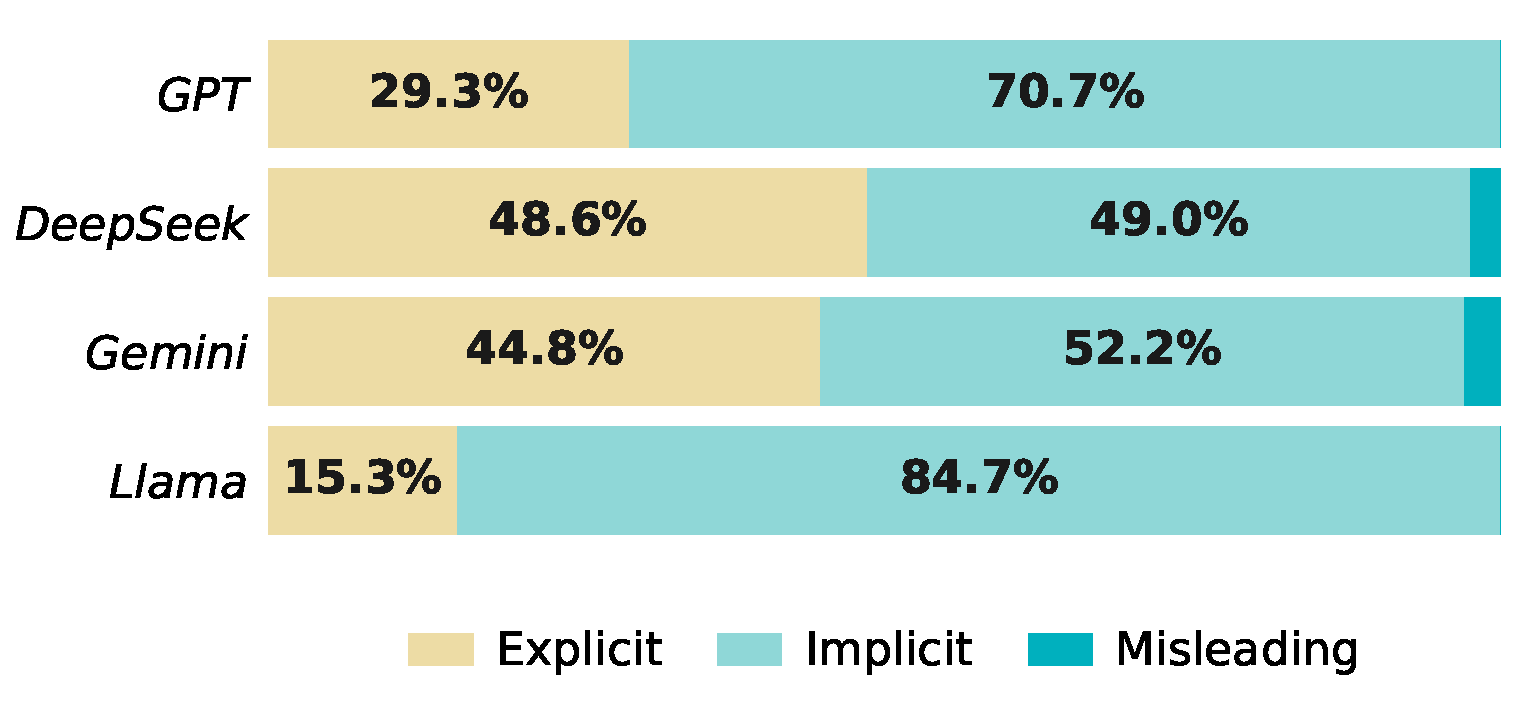
\includegraphics[width=1\linewidth]{Figures/noisy_tool_behavior_inner_bar.pdf}
    \vspace{-0.35in}
    \caption{Distribution of invoked block alternatives under \textit{mixed} blocking. For each model, the horizontal bar normalizes all invoked block alternatives to $100\%$. Colors indicate whether the invoked block alternative is an explicit failure, implicit failure, or semantic misleading tool. We abbreviate \textit{GPT-5.4}, \textit{Gemini-3.5-Flash}, \textit{DeepSeek-V4-Flash}, and \textit{Llama-3.3-70B-Instruct} as \textit{GPT}, \textit{Gemini}, \textit{DeepSeek}, and \textit{Llama}.}
    \label{fig:noisy_tool_type_mix}
    % \vspace{-0.2in}
\end{figure}

% \begin{figure}[t]
    \centering
    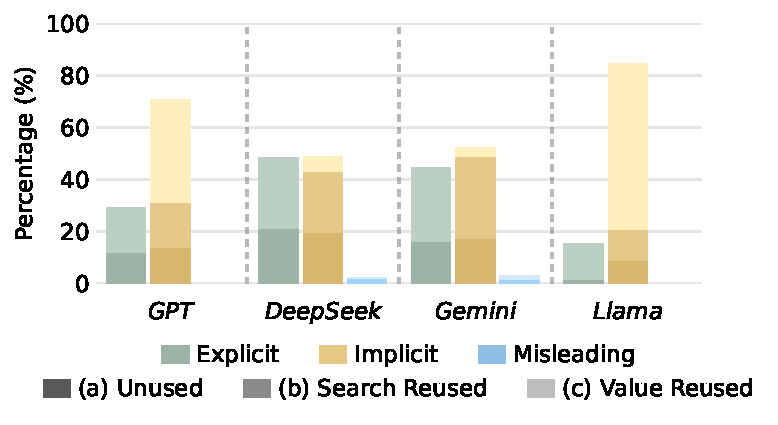
\includegraphics[width=1\linewidth]{Figures/noisy_tool_behavior_outer_bar_vertical.pdf}
    \vspace{-0.35in}
    \caption{Follow-up behavior after agents invoke block alternatives under \textit{mixed} blocking. Each colomn corresponds to one model and one block type. The row length shows the ratio of all invoked block alternatives for that model, and colored segments denote \textit{Unused}, \textit{Search Reused}, and \textit{Value Reused}. \textit{GPT} denotes \textit{GPT-5.4}, \textit{Gemini} denotes \textit{Gemini-3.5-Flash}, \textit{DeepSeek} denotes \textit{DeepSeek-V4-Flash}, and \textit{Llama} denotes \textit{Llama-3.3-70B-Instruct}.}
    \label{fig:noisy_tool_followup_behavior}
    \vspace{-0.2in}
\end{figure}

% \paragraph{Models can often avoid semantically misleading tools, but still continue from explicit or implicit failures.}
% Figures~\ref{fig:noisy_tool_type_mix} and~\ref{fig:noisy_tool_followup_behavior} analyze agents' behavior after they invoke block alternatives returned under retrieval-time blocking.
% Here, blocked alternatives refer to the additional tools inserted in place of blocked executable tools.
% Figure~\ref{fig:noisy_tool_type_mix} shows which type of blocked alternative each model invokes.
% Figure~\ref{fig:noisy_tool_followup_behavior} further shows how agents use the output of each invoked block alternative in later steps.
% We categorize follow-up behavior into three cases:
% \begin{itemize}[topsep=2pt, partopsep=3pt, leftmargin=*, itemsep=-3pt]
%     \item \textbf{\textit{Unused}}: the agent uses neither the tool's output datatype for later retrieval nor its returned value in a later tool call.
%     \item \textbf{\textit{Search Reused}}: the agent uses the tool's output datatype to retrieve further tools, but does not use its concrete returned value as an argument in a later tool call.
%     \item \textbf{\textit{Value Reused}}: the agent uses the tool's concrete returned value as an argument in a later tool call, where the called tool may have been retrieved either before or after this additional tool was invoked.
% \end{itemize}

% Across models, agents invoke explicit failure and implicit failure tools much more often than semantic misleading tools. 
% Semantic misleading tools account for at most $3\%$ of invoked block alternatives, and are never selected by \textit{GPT-5.4} or \textit{Llama-3.3-70B-Instruct}.
% This suggests that models can often use tool names and descriptions to avoid tools whose functions are only superficially related to the current need.
% However, they still struggle with blocked alternatives whose schema and task intent look relevant but whose execution is unavailable or unreliable.

% % The more prominent failure pattern concerns how agents behave after invoking explicit or implicit failure tools.
% Agents show different follow-up behavior after receiving outputs from explicit failure tools and implicit failure tools.
% After invoking explicit-failure blocked alternatives, agents never use the returned error message as an argument in later tool calls.
% They either stop using the result, or use only the tool's declared output datatype to search for downstream tools.
% This shows that explicit errors usually stop direct value propagation, but they do not always stop agents from continuing to search from the failed tool's declared output type.
% Implicit-failure blocked alternatives are harder to handle because they return plausible concrete values instead of explicit errors.
% For \textit{GPT-5.4} and \textit{Llama-3.3-70B-Instruct}, \textit{Value Reused} accounts for $55.9\%$ and $75.5\%$ of implicit-failure follow-ups, respectively.
% Aggregated across models, implicit failures lead to \textit{Value Reused} in $42.2\%$ of cases, compared with $0\%$ for explicit failures.
% This shows that silent failures can inject invalid intermediate values that agents carry into later tool calls, making the failure harder to detect and contain.

% \qh{need to check the sign consistency}
% \subsection{Definitions}
% \label{sec:mechanistic-error-definitions}

% % % \begin{table*}[t]
% % \centering
% % \small
% % \setlength{\tabcolsep}{5pt}
% % \begin{tabular}{lccccc}
% % \toprule
% % \textbf{Model}
% % & \textbf{Failed runs}
% % & \textbf{No Traction}
% % & \textbf{Irrecoverable Drift}
% % & \textbf{Weak Recovery}
% % & \textbf{Interaction Breakdown} \\
% % \midrule
% % \textit{GPT-5.4} & 152 & 7.2 & 69.1 & 5.9 & 13.2 \\
% % \textit{DeepSeek-V4-Flash} & 120 & 2.5 & 21.7 & 3.3 & 71.7 \\
% % \textit{Gemini-3.5-Flash} & 153 & 13.1 & 60.1 & 3.3 & 7.8 \\
% % \textit{Llama-3.3-70B-Instruct} & 265 & 10.9 & 35.1 & 0.4 & 52.5 \\
% % \midrule
% % \textbf{All models} & 690 & 9.1 & 45.8 & 2.8 & 37.2 \\
% % \bottomrule
% % \end{tabular}
% % \caption{Default-setting trajectory failure categories (\% of failed runs). A successful call is counted as progress if it produces a new intermediate value needed by at least one valid tool-use path toward the final answer.}
% % \label{tab:mechanistic_navigation_breakdown}
% % \end{table*}

% \begin{table*}[t]
% \centering
% \small
% \setlength{\tabcolsep}{5pt}
% \resizebox{\linewidth}{!}{
% \begin{tabular}{llcccccc}
% \toprule
% \multirow{2}{*}{\textbf{Model}}
% & \multirow{2}{*}{\shortstack{\textbf{Dominant}\\\textbf{Ending}}}
% & \multicolumn{2}{c}{\textbf{\# Non-interaction Failures}}
% & \multicolumn{2}{c}{\textbf{Dominant Ending Ratio (\%)}}
% & \multicolumn{2}{c}{\textbf{Failure-only S/C Ratio}} \\
% \cmidrule(lr){3-4}
% \cmidrule(lr){5-6}
% \cmidrule(lr){7-8}
% & &
% \textbf{Default} & \textbf{Blocker} & \textbf{Default} & \textbf{Blocker} & \textbf{Default} & \textbf{Blocker} \\
% \midrule
% \textit{GPT-5.4}
% & Surrender & 132 & 139 & 77.3 & 80.6 & 4.5 & 4.2 \\
% \textit{DeepSeek-V4-Flash}
% & Wrong tool value & 34 & 44 & 58.8 & 65.9 & 6.1 & 4.6 \\
% \textit{Gemini-3.5-Flash}
% & Search exhaustion & 141 & 154 & 90.8 & 85.1 & 29.1 & 18.3 \\
% \textit{Llama-3.3-70B}
% & Wrong tool value & 126 & 106 & 81.7 & 71.7 & 2.1 & 2.0 \\
% \bottomrule
% \end{tabular}
% }
% \caption{
% The most frequent ending type for each model after planning failures.
% \emph{\# Non-interaction Failures} is the number of failures after excluding interaction breakdowns in the corresponding setting.
% \emph{Dominant Ending Ratio} is the share of those failures that end with the behavior named in the second column.
% \emph{Failure-only S/C Ratio} is the average S/C Ratio computed only over the non-interaction failure traces.
% \jy{check this table}
% }
% \label{tab:mechanistic_termination_behavior}
% \end{table*}

% \paragraph{\textbf{Progress is defined by distance reduction in the datatype graph.}}
% For each query, let $T$ denote the target datatype and let $S_t$ denote the set of datatypes whose values the model has obtained before step $t$.
% We compute $d(x,T)$ as the shortest directed distance from datatype $x$ to $T$ in the baseline tool graph, and define the model's best current position as $\min_{x \in S_t} d(x,T)$.
% A successful tool call with output datatype $y$ is a \emph{progress call} if $d(y,T) < \min_{x \in S_t} d(x,T)$; otherwise it is a \emph{non-progress call}.
% This definition rewards any path that moves structurally closer to the target, rather than requiring the model to follow one fixed ground-truth shortest path.

% \paragraph{\textbf{Navigation failures are grouped into three graph-level categories.}}
% \emph{No Traction} means the failed trajectory never makes a progress call.
% \emph{Irrecoverable Drift} means the model makes at least one progress call, then makes a non-progress call, and never makes progress again.
% \emph{Weak Recovery} means the model makes progress after a non-progress call, but still fails before reaching a correct answer.
% These categories identify where the trajectory breaks in the tool graph: before entering a useful path, after drifting away from it, or after a shallow recovery that does not finish the task.

% \paragraph{\textbf{Interaction breakdown is separated from graph-navigation failure.}}
% \emph{Interaction Breakdown} covers failures caused by protocol, retrieval, label, tool-call, or resource-level errors, such as exceeding the maximum number of invalid tool calls.
% We report this category separately because it reflects the model's ability to follow the environment interface, not its ability to choose a structurally useful next tool.
% This separation keeps the main navigation analysis focused on recoverability and tool selection rather than format compliance.

% \paragraph{\textbf{Cross-setting drift is measured by total variation distance over failure categories.}}
% For each model and setting, let $p_s(c)$ be the percentage of failed runs assigned to failure category $c \in \mathcal{C}$, where $\mathcal{C}$ includes \emph{No Traction}, \emph{Irrecoverable Drift}, \emph{Weak Recovery}, \emph{Interaction Breakdown}, and \emph{Residual}.
% We define the drift from the default setting as
% \[
% \mathrm{TVD}(s,\mathrm{default}) = \frac{1}{2}\sum_{c \in \mathcal{C}} \left|p_s(c) - p_{\mathrm{default}}(c)\right|.
% \]
% Because $p_s(c)$ is measured in percentage points, TVD is also reported in percentage points and ranges from $0$ to $100$.
% This metric captures how much the full failure distribution changes under an intervention, rather than only whether the most frequent category changes.

% \paragraph{\textbf{Termination behavior is analyzed separately from failure mechanism.}}
% After a navigation failure, different models may produce different final behaviors: they may explicitly surrender, commit a wrong value returned by a tool, confabulate a value, or continue searching without an answer.
% We treat these as \emph{termination behaviors}, not as primary failure mechanisms, because the same graph-level failure can end in different surface outputs.
% This lets us ask two distinct questions: where the tool trajectory breaks, and how each model behaves after it can no longer ground the target answer.

% \subsection{Main Findings}
% \label{sec:mechanistic-error-findings}

% \begin{takeaway}
% Most non-protocol failures arise from biased tool selection after the model leaves a progress path, and recovery is weak.
% \end{takeaway}

% \paragraph{\textbf{Models usually fail after drifting away from a progress path.}}
% Table~\ref{tab:mechanistic_navigation_breakdown} shows that \emph{Irrecoverable Drift} is the largest non-interaction failure pattern in the default setting for GPT-5.4 and Gemini-3.5-Flash, accounting for $69.1\%$ and $60.1\%$ of their failures, respectively.
% Aggregated across all four models, irrecoverable drift accounts for $45.8\%$ of default failures, while \emph{Weak Recovery} accounts for only $2.8\%$.
% This means that models do sometimes enter useful tool paths, but once they make a non-progress call, they rarely recover enough to finish the task.

% \paragraph{\textbf{The failure is usually not that a progress tool was never retrieved.}}
% Table~\ref{tab:mechanistic_search_opportunity} shows that before failed-run non-progress calls, a clean progress-capable baseline tool was already in the model's retrieved tool history in $78.0\%$ of default cases and $71.1\%$ of blocker cases.
% Thus, many wrong calls occur despite a structurally useful alternative being available in the model's prior search results.
% This supports a selection-failure interpretation: the model often sees a tool that could reduce distance to the target, but chooses a different tool.

% \paragraph{\textbf{Models exhibit a recency bias that makes backtracking difficult.}}
% Table~\ref{tab:mechanistic_search_opportunity} shows that in the default setting, $74.1\%$ of non-progress calls use tools from the current or immediately previous retrieval window, while $44.7\%$ of clean progress opportunities involve a progress tool that is more than two retrieval windows old.
% The blocker setting shows the same pattern: $63.6\%$ of non-progress calls use recent tools, while $43.2\%$ of clean progress opportunities are old.
% At the same time, clean progress tools reappear after drift in $42.5\%$ of default opportunities and $53.4\%$ of blocker opportunities, so the issue is not only memory loss.
% Recovery is difficult because models both underuse older useful tools and fail to select progress tools even when those tools re-enter the recent search context.

% \begin{takeaway}
% After navigation failure, models terminate in different characteristic ways: GPT surrenders, DeepSeek and Llama commit wrong tool values, and Gemini keeps searching.
% \end{takeaway}

% \paragraph{\textbf{GPT-5.4 usually recognizes that it cannot ground the answer and explicitly surrenders.}}
% Table~\ref{tab:mechanistic_termination_behavior} reports termination behavior after excluding interaction-level failures.
% In the default setting, GPT-5.4 ends $77.3\%$ of its non-interaction failures with an explicit surrender statement; in the blocker setting, this rises to $80.6\%$.
% This indicates that GPT's dominant post-failure behavior is conservative: once its tool trajectory stops producing grounded progress, it tends to refuse to fabricate a concrete answer.

% \paragraph{\textbf{DeepSeek and Llama more often commit values from the wrong branch.}}
% Table~\ref{tab:mechanistic_termination_behavior} shows that DeepSeek-V4-Flash commits wrong tool-returned values in $58.8\%$ of default non-interaction failures and $65.9\%$ of blocker failures.
% Llama-3.3-70B shows the same tendency more strongly, committing wrong tool values in $81.7\%$ of default failures and $71.7\%$ of blocker failures.
% These models therefore fail less by refusing to answer and more by treating off-path observations as sufficient evidence.

% \paragraph{\textbf{Gemini's characteristic failure is continued search without commitment.}}
% Table~\ref{tab:mechanistic_termination_behavior} shows that Gemini-3.5-Flash ends $90.8\%$ of default non-interaction failures and $85.1\%$ of blocker failures through search exhaustion.
% Its search-to-call ratio is also much larger than the other models: $29.1$ in default and $18.3$ in blocker.
% This suggests that Gemini's failure policy is not premature commitment, but an inability to convert search into decisive progress once it loses the path.

% \begin{takeaway}
% Experimental settings mostly change failure severity, not each model's dominant failure fingerprint.
% \end{takeaway}

% \paragraph{\textbf{Across settings, most models preserve their dominant failure type.}}
% Table~\ref{tab:mechanistic_cross_setting_drift} compares each model's failure distribution in every non-default setting against its default distribution using total variation distance over all failure categories.
% DeepSeek-V4-Flash, Gemini-3.5-Flash, and Llama-3.3-70B never change their dominant failure category across the $11$ non-default settings.
% This shows that settings such as blocking, noise type, path ratio, and path length generally amplify existing weaknesses rather than creating new failure modes.

% \paragraph{\textbf{GPT-5.4 is the main model whose dominant failure type changes under harder settings.}}
% Table~\ref{tab:mechanistic_cross_setting_drift} shows that GPT-5.4 changes its dominant failure type in $2$ of $11$ non-default settings.
% In default, GPT-5.4 is dominated by irrecoverable drift ($69.1\%$ in Table~\ref{tab:mechanistic_navigation_breakdown}); under blocker and feedback, interaction breakdown becomes dominant, with feedback producing the largest distribution shift (TVD $64.0$).
% This exception suggests that harder settings can push GPT from navigation failure into repeated invalid tool-call behavior, but this shift is not the general pattern across models.

% \paragraph{\textbf{Path and blocking interventions primarily modulate difficulty rather than behavior type.}}
% Table~\ref{tab:mechanistic_cross_setting_drift} shows moderate median drift for Gemini ($20.4$ TVD) and Llama ($13.0$ TVD), and low median drift for DeepSeek ($9.5$ TVD), despite these settings changing path availability, blocker behavior, and path length.
% The dominant failure type remains stable even when the total failure rate changes.
% This means the benchmark conditions act mainly as stress tests for each model's existing failure policy, not as separate tasks that induce unrelated errors.

% \subsection{Implications}
% \label{sec:mechanistic-error-implications}

% \paragraph{\textbf{The resulting picture is hierarchical.}}
% At the trajectory level, models fail because they select non-progress tools and rarely recover after drift; at the model level, they expose this failure through different termination behaviors; at the setting level, interventions mostly change how often each model's existing failure pattern appears.
% Together, Tables~\ref{tab:mechanistic_navigation_breakdown}--\ref{tab:mechanistic_cross_setting_drift} support a single account: tool-use failures are governed by structural navigation limits, model-specific stopping policies, and setting-dependent stress.
% This hierarchy gives us a cleaner target for future interventions: improve structural tool selection and recovery first, then tune model-specific stopping behavior. 

% \paragraph{\textbf{Better benchmark performance requires structural tool selection.}}
% Table~\ref{tab:mechanistic_search_opportunity} shows that progress-capable tools are often already present in the retrieved history when the model makes a non-progress call.
% This implies that simply increasing retrieval volume or turn budget is unlikely to solve the dominant failure mode.
% Future agents should explicitly track graph progress, preserve useful earlier candidates, and re-rank tools by whether they reduce distance to the target.

% \paragraph{\textbf{Model-specific termination biases disrupt the exploration--execution feedback loop in different ways.}}
% Table~\ref{tab:mechanistic_termination_behavior} shows that GPT-5.4 often surrenders despite retaining substantial interaction budget, suggesting insufficient exploration tendency; DeepSeek and Llama more often commit incorrect tool values, suggesting overconfident execution under uncertainty; and Gemini repeatedly searches without committing to execution, suggesting difficulty transitioning from information gathering to action. These patterns show that agent failure is not only about whether a model can find the right information, but also about whether it can decide when to keep exploring, when to express uncertainty, and when to execute partial progress to obtain new feedback.